\section{Introducción}
En el ámbito universitario resulta necesario mantener informadas a las personas sobre una amplia variedad de hechos, noticias y acontecimientos que sucedieron o sucederán, desde la ubicación de un aula hasta la notificación de la cancelación de una clase. Muchas veces estas notificaciones son sobre cuestiones muy efímeras, lo que requiere rapidez para empezar a transmitirlas y facilidad para tener el alcance necesario.

En las facultades de la Universidad Nacional de La Plata se consumen muchos recursos para cumplir este fin, a través de afiches, pancartas, panfletos, etc. los cuales, pese a ser de barata fabricación, no tienen una vida útil muy extensa. Además todas estas formas de comunicación se basan en el uso de papel, que tras ser utilizado debe desecharse debido a la imposibilidad de reutilizarlo, generando una cantidad de residuos significativa. Si se tiene en cuenta que también generan una polución visual considerable, por la gran cantidad de estos distribuidos en todos los lugares transitables, resulta prudente considerar una nueva forma de comunicación.

% TODO: Mencionar sobre otros carteles comercialmente disponibles
Existen en el mercado varios carteles electrónicos capaces de visualizar mensajes simples, con la particularidad de que suelen requerir que el mensaje sea cambiado manualmente accediendo fisicamente al cartel, lo cual resulta arriesgado al tener en cuenta que este cartel estará en espacios concurridos por cientos de personas.

Surge así la idea de desarrollar un cartel electrónico, capaz de ser configurado de forma remota y unicamente por las autoridades competentes, con el fin de proveer una forma de comunicación masiva más limpia, clara y menos dañina para el medio ambiente.

En este informe se describe todas las fases del desarrollo de un proyecto para la asignatura Taller de Proyecto 1. El trabajo consiste en el diseño y desarrollo de un cartel luminoso cuyo contenido es configurable de forma remota. El cartel cuenta con conectividad WiFi, con lo que es capaz de formar parte de una red IP.

De esta forma, a través de una aplicación de PC, se puede establecer, de manera remota, el contenido del cartel. Cabe destacar que el programa de PC también es competencia de este proyecto, habiendo sido desarrollado en su totalidad por los integrantes del mismo.

Por otra parte, se requiere que el mensaje a mostrar, sólo pueda ser manipulado por las personas autorizadas a operar el sistema. Para ello, el mismo debe brindar seguridad a los usuarios utilizando credenciales para ingresar a la red WiFi, una contraseña de acceso al sistema y un mecanismo de encriptación de los paquetes intercambiados entre la aplicación de PC y el cartel.

A lo largo de este informe se documentan las fases de desarrollo previamente mencionadas.

En la sección \ref{part:analisis} se habla sobre los requerimientos y especificaciones del sistema, detallando que funcionalidades debe tener y a cuáles restricciones está sujeto.

Luego, en la sección \ref{part:diseno}, se mencionan las componentes que constituyen el sistema, se explicitan modelos que describen el comportamiento del mismo, la interfaz de usuario y la arquitectura del software. También se muestran los esquemáticos que especifican la conexión de los componentes.

En la sección de implementación se describe el proceso de desarrollo de software, tanto del código que corre sobre el microcontrolador que gobierna el cartel así como también la aplicación de PC. 
Adicionalmente se detalla la implementación física del prototipo.

En la sección de ensayos se documenta los resultados de las pruebas que se realizaron sobre el sistema en funcionamiento.

Por último, se anexa como apéndice un detalle del presupuesto requerido para la realización del proyecto, más una guía instructiva que explica los pasos necesarios para poner en marcha el sistema, junto a más piezas de información que el equipo considera de interés para el entendimiento pleno del proyecto y de su implementación.


\section{Objetivos del proyecto}
El objetivo primario de este proyecto es el diseño e implementación de un cartel luminoso que pueda ser configurado remotamente por los usuarios.
La configuración se realiza a través de una aplicación de PC que también es competencia de este proyecto. 
No se tiene como finalidad realizar un producto diseñado de manera que sea económicamente viable producirlo en masa, sino más bien el desarrollo de un prototipo a modo de prueba de concepto. 
Es necesario que el sistema a desarrollar responda a diferentes necesidades de operabilidad, conectividad, funcionamiento y seguridad que se detallan a lo largo del presente informe.

El proyecto se divide en los siguiente módulos de desarrollo:

\begin{itemize}
	\item Hardware del cartel.
	\item Software de la aplicación de PC.
	\item Sofware del microcontrolador que controla el cartel.
	\item Protocolo de comunicación de red por medio del cual interactuarán los módulos de software previamente enunciados
\end{itemize}


\section{Filosofía de diseño} \label{sec:filosofia}
El proyecto se basa en un proceso de desarrollo de cascada, como se muestra en la figura \ref{fig:waterfall}. Este diagrama se corresponde con la filosofía \emph{topdown}. A lo largo de esta sección se explica en qué consiste cada una de las etapas que se presentan.

\begin{figure}[!ht]
	\centering
	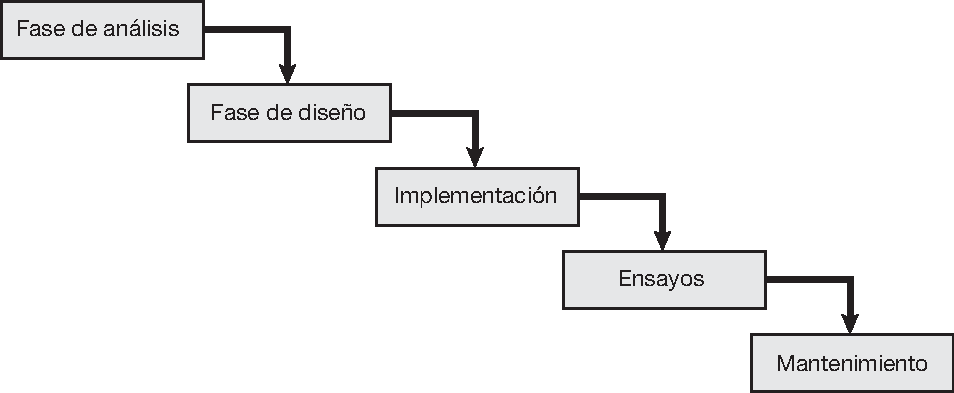
\includegraphics[width=1\linewidth]{imagenes/waterfall.pdf}
	\caption{Modelo en cascada de desarrollo.}
	\label{fig:waterfall}
\end{figure}


\subsection{Análisis}
En la fase de análisis, se realiza una elicitación de los requerimientos que tiene el sistema, lo que permite obtener especificaciones detalladas del producto a construir tales como sus dimensiones y consumo energético. Por otro lado, también se determinan sus restricciones relacionadas con el costo, la seguridad y la compatibilidad con otros sistemas con los que éste interactúa.

Por este motivo, en esta primera etapa es necesario considerar tanto el peso y tamaño del prototipo así como el consumo de energía del mismo, necesaria para operar el sistema.

Adicionalmente se debe analizar su costo de producción y el tiempo de desarrollo necesario para ponerlo en marcha.


\subsection{Diseño}
En la fase de diseño se realizan los diagramas en bloques tanto de la arquitectura de software como de hardware. Además se realizan esquemas, UMLs, diagramas de flujos, de estados y la construcción de un modelo conceptual del sistema.

En esta etapa se determina la plataforma de hardware entre las que se encuentran microcontroladores, FPGAs, DSPs, entre otros y la plataforma de software que abarca desde el lenguaje a utilizar, así como también los frameworks, y demás herramientas que se utilizarán en el desarrollo del proyecto.

Adicionalmente, en la etapa de diseño, se procede a realizar la división del sistema en módulos, en capas y en tareas que se reparten a los integrantes del grupo. También se diseñan los esquemáticos de las componentes y la interconexión entre ellas.


\subsection{Implementación}

En la fase de implementación se desarrolla el firmware, se compilan y se debuguean los programas en busca de errores que pudieron surgir a lo largo de la programación del software. También se confecciona la PCB y se sueldan las componentes sobre ella.


\subsection{Ensayos}
En la fase de ensayos se validan todas las funcionalidades del sistema y se realizan mediciones de perfomance globales, en relación al consumo, utilización de recursos, velocidad y memoria.

Además se realiza la revisión general del producto evaluando la conformidad del cliente.

Una posibilidad para realizar este proceso, es listar todos los requerimientos del sistema y demostrar que el producto realizado cumple con cada uno de ellos.


\subsection{Mantenimiento}
Una vez que el producto es entregado al cliente, la última etapa se conoce como mantenimiento.
En ella se corrigen los errores o bugs que puedan llegar al surgir al utilizar el producto.

Por otra parte, se le añaden nuevas funcionalidades de acuerdo a las posteriores necesidades del cliente.
Para realizar este proceso, es indispensable redactar una nueva especificación de requerimientos en donde se detalle la nueva funcionalidad y el tiempo estimado de desarrollo de la misma.

Opcionalmente se puede migrar hacia otro hardware más veloz o de menor consumo según fuese necesario adaptándolos a otros ambientes de operación.
